\section{Dynamic neural scene representation}

\paragraph{Problem statement} 
Consider a set of LiDAR scans $\mathcal{X} = \{\mathbf{X}_t\}_{t=1}^T$ that have been compensated for ego-motion, along with tracked bounding boxes\footnote{We assume that the ground truth object detection and tracking annotations are available.} for dynamic vehicles $\mathcal{B} = \{\mathbf{B}_t^v\}_{v=1}^{N}$, where $T$ represents the total number of LiDAR scans, and $N$ is the count of dynamic vehicles. Each scan $\mathbf{X}_t$ is composed of $n_t$ rays, each ray $\mathbf{r}$ is described by the tuple $(\origin, \dir, \zeta, \intensity, \pdrop)$, where $\origin$ and $\dir$ denote the ray's origin and direction, $\zeta$ and $\intensity$ represent range and intensity values, and $\pdrop \in \{0,1\}$ indicates whether the ray is dropped or not due to insufficient returned radiant power.


The goal is to reconstruct the scene with a static-dynamic decomposed neural representation, that can enable the rendering of LiDAR scan $\mathbf{X}_{\text{tgt}}$ from novel viewpoint $\mathbf{T}_{\text{tgt}}$. This setup also facilitates various object manipulations, including altering object trajectories, and inserting or removing objects from the scene. The overview of our method is given in~\cref{fig:main}.

\subsection{Neural scene decomposition} \label{sec: decomposition}
We leverage the inductive bias that driving scenes can be decomposed into a static component and $N$ rigidly-moving dynamic components~\cite{huang2022dynamic,gojcic2021weakly}. Consequently, we establish $N+1$ neural fields. The neural field $\mathbf{F}_{\text{static}}$ is designated for the static component of the scene, capturing the unchanging background elements. Concurrently, the set of neural fields $\{\mathbf{F}^v\}_{v=1}^{N}$ is used to model the $N$ dynamic entities, specifically the vehicles in motion.



\paragraph{Neural field for static background} 
The static background is encoded into a neural field $\mathbf{F}_\text{static}: (\x, \dir) \mapsto (s, \intensity, \pdrop)$ that estimates the signed distance $s$, intensity $\intensity$, and ray drop probability $\pdrop \in [0,1]$ given the point coordinates $\x$ and the ray direction $\dir$. In practice, we first use a multi-resolution hash encoding (MRH)~\cite{mueller2022instant} to map each point to its positional feature $\posfeat \in \real^{32}$, and project the view direction onto the first 16 coefficients of the spherical harmonics basis, resulting in $\dirfeat$. Subsequently, we utilize three Multilayer Perceptrons (MLPs) to estimate the scene properties as follows:
\begin{equation}
(s, \geofeat) = f_s(\posfeat), \quad \intensity = f_{\intensity}(\rayfeat), \quad \pdrop = f_{\text{drop}}(\rayfeat).
\end{equation}
Here, $f_s, f_e,$ and $f_{\text{drop}}$ are three MLPs, $\rayfeat \in \mathbb{R}^{31}$ represents the ray feature and is constructed by concatenating the per-point geometric feature and the directional feature. The geometric feature is denoted as $\geofeat \in \mathbb{R}^{16}$. For more implementation details, please refer to the appendix. 

\begin{figure}[t]
    \centering
        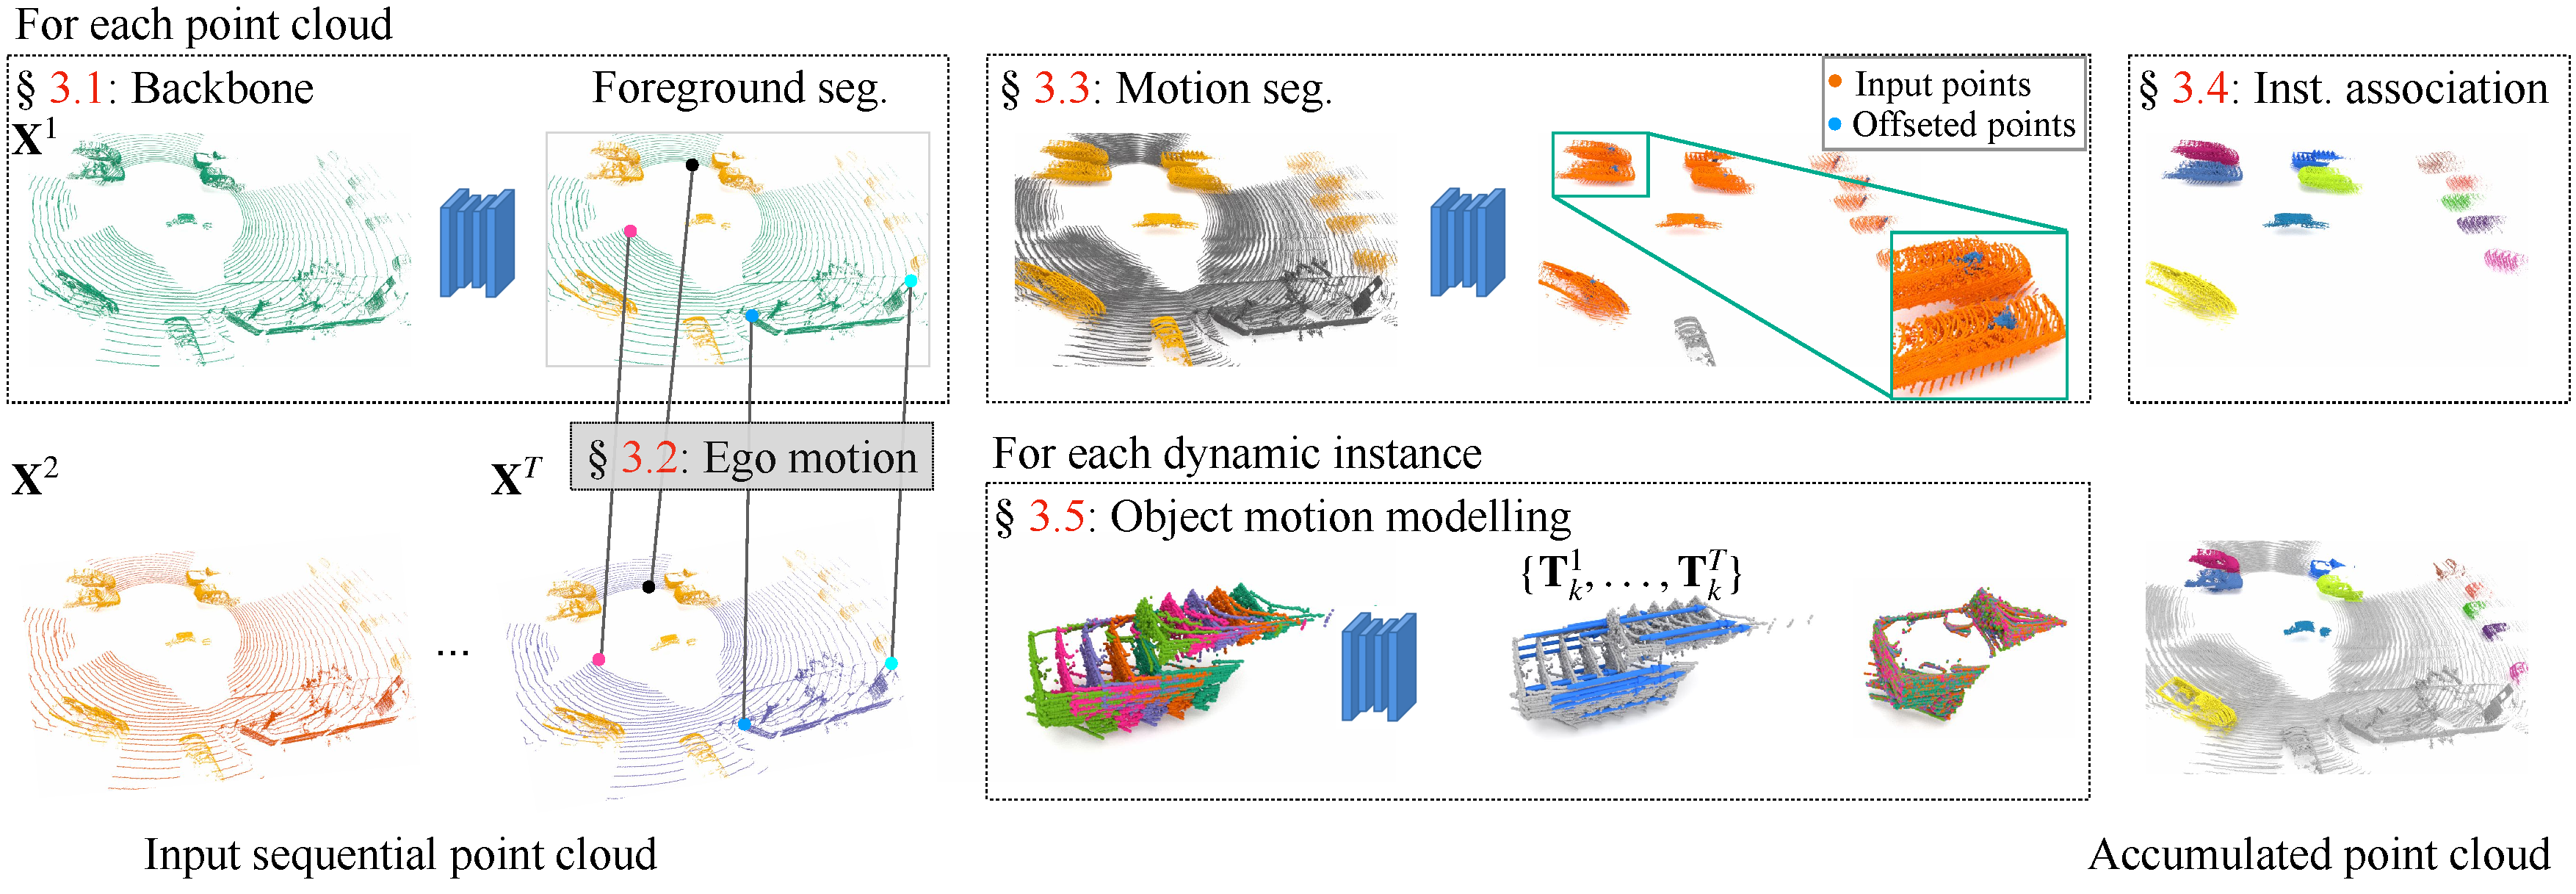
\includegraphics[width=1.0\columnwidth]{Figures/overview.pdf}
        \caption{
        Overview of \dynfl. Our method takes LiDAR scans and tracked bounding boxes of dynamic vehicles as input. \dynfl first decomposes the scene into a static background and $N$ dynamic vehicles, each modelled using a dedicated neural field. These neural fields are then composed to re-simulate LiDAR scans in dynamic scenes. Our composition technique supports various scene edits, including altering object trajectories, removing and adding reconstructed neural assets between scenes.
    }
    \label{fig:main}
\end{figure}


\paragraph{Neural fields for dynamic vehicles} 
LiDAR scans collected over time are often mis-aligned due to the motion of both the sensor and other objects in the scene. Despite applying ego-motion for aligning static background points, dynamic object points remain blurred along their trajectories. Our approach to constructing a dynamic neural scene representation is grounded in the assumption that each dynamic object only undergoes rigid motion. Therefore, we can first align them over time and reconstruct them in their \textit{canonical} coordinate frame, and then render them over time by reversing the alignment of the neural field.

Specifically, consider a dynamic vehicle $v$ 
occurring in LiDAR scans $\{\mathbf{X}^v_t\}_{t=1}^{T}$ along with the associated bounding boxes $\{\mathbf{B}^v_t \in \mathbb{R}^{3\times 8}\}_{t=1}^{T}$ in the world coordinate framework. Here each bounding box is defined by its eight corners, and the first bounding box $\mathbf{B}^v_1$ is considered as the \textit{canonical} box. We estimate the relative transformations $\{\mathbf{T}_t \in \text{SE}(3)\}_{t=2}^{T}$ between the remaining $T-1$ bounding boxes and the canonical box, expressed as $\mathbf{B}_1^v = \mathbf{T}_t \mathbf{B}_t^v$\footnote{$\mathbf{T}\mathbf{B} = \mathbf{R}\mathbf{B} + \mathbf{t}$, where $\mathbf{R}$ and $\mathbf{t}$ are the rotation and translation components of $\mathbf{T}$.}. 
Subsequently, all LiDAR measurements on the object are transformed and accumulated in its canonical coordinate frame. The vehicle $v$ is then reconstructed in its canonical space, akin to the static background, using a neural field $\mathbf{F}^v$. To render the dynamic vehicle at timestamp $t$, the corresponding rigid transformation is applied to the queried rays. The dynamic neural field can thus be expressed as: $\mathbf{F}^v_t: (\mathbf{T}_{t}\x, \mathbf{T}_{t}\dir) \mapsto (s, \intensity, \pdrop)$. The rendering process for $\mathbf{F}^v$ is the same as rendering for static neural field $\mathbf{F}_{\text{static}}$.


